\section{基于概率的分类}
\label{sec:classification-probability}

第\ref{sec:classic-overview-probabilistic}节已区分直接建立条件类别概率与先描述类条件输入分布的两条路线。本节分别用Logistic回归、朴素贝叶斯和GDA说明参数估计、类别决策与概率检验。沿用训练集$D_n$，类别数为$C$、类别索引为$c$；$p$按观测类型表示概率质量函数或概率密度。LDA的共享协方差推导见第\ref{sec:classification-lda}节，这里直接在一般高斯模型族中使用该结果。

\subsection{Logistic 回归}
\label{sec:classification-logistic}

若直接用实值线性函数拟合$0/1$标签，输出可能小于零或大于一，不能直接解释为概率。\term{Logistic回归}（logistic regression）保留线性得分，却通过一个有界变换把它映射为正类概率。这里将二分类标签约定为$\{0,1\}$；名称中的“回归”描述对概率与特征关系的建模，任务仍是分类。

第\ref{sec:regression-glm}节把伯努利分布、logit链接与其他响应模型统一在广义线性模型中；本节复用这套条件概率结构，但进一步规定类别决策阈值与误判代价，并单独检查概率校准。

Logistic曲线的历史早于统计分类。Verhulst在1838年用它描述受增长上限约束的人口变化，后来这一曲线进入生物测定和二值响应分析。从增长曲线到统计回归，函数保留了相同形式，变量与参数的解释却发生了变化；Cramer对这一发展过程作了专门考证\scite{cramer2002origins}

\subsubsection{模型结构}
\label{sec:classification-logistic-structure}

记$p(\bm{x})=\mathbb{P}(y=1\mid\bm{x})$。比值$p(\bm{x})/[1-p(\bm{x})]$称为\term{几率}（odds），衡量正类相对于负类的可能性。对它取对数得到\term{对数几率}（log-odds，也称logit），其取值可以覆盖整个实数轴，因而适合与线性得分连接：
\begin{equation}
  \label{eq:classification-logistic-logodds}
  \log\frac{p(\bm{x})}{1-p(\bm{x})}
  =\bm{w}^{\top}\bm{x}+b.
\end{equation}
其中$\bm{w}\in\mathbb{R}^{d}$是权重，$b\in\mathbb{R}$是偏置。令右侧为$z$，由$p/(1-p)=e^z$整理出$p=e^z/(1+e^z)$，便得到
\begin{equation}
  \label{eq:classification-logistic-sigmoid}
  p(\bm{x})=\sigma(\bm{w}^{\top}\bm{x}+b),
  \qquad
  \sigma(z)=\frac{1}{1+e^{-z}}.
\end{equation}
这个S形函数称为\term{Sigmoid函数}（sigmoid function），此处特指Logistic形式。它把任意有限得分转成严格介于零和一之间的数。Cox在1958年的二值序列回归研究是这一统计建模路线的经典文献\scite{cox1958binary}

参数的解释落在对数几率尺度上：保持其他特征不变，$x_j$增加一个单位，正类几率乘以$e^{w_j}$。概率本身的变化还取决于原来的概率，因为
\[
  \frac{\partial p(\bm{x})}{\partial x_j}
  =w_jp(\bm{x})[1-p(\bm{x})].
\]
因此，$w_j$的正负说明模型中的影响方向，大小却不能脱离特征单位直接比较，也不自动具有因果含义。例如，假设某特征的$w_j=\log 2$，原来正类概率为$1/2$，该特征增加一单位后概率变为$2/3$，而不是增加固定的$\log 2$。

在两类误判代价相同时，以$p(\bm{x})\geq1/2$预测正类，边界就是$\bm{w}^{\top}\bm{x}+b=0$。若误报的代价为$a>0$、漏报为$r>0$，正确分类代价为零，则预测正类的条件是$a[1-p(\bm{x})]\leq rp(\bm{x})$，即阈值改为$a/(a+r)$。这一决策解释要求输入概率足够可靠；合法的数值范围本身还不能保证这一点。

图\ref{fig:classification-logistic-probability}把概率阈值与得分阈值放在同一条曲线上比较。一般地，概率阈值$\tau\in(0,1)$对应得分阈值$\log[\tau/(1-\tau)]$。在图中的教学设定下，误报与漏报代价相等时取$\tau=0.5$；若改成$a=4$、$r=1$，则$\tau=0.8$，得分至少达到$\log4\approx1.386$才预测正类。曲线本身没有改变，改变的是把概率转成类别的规则。
\begin{figure}[htbp]
  \centering
  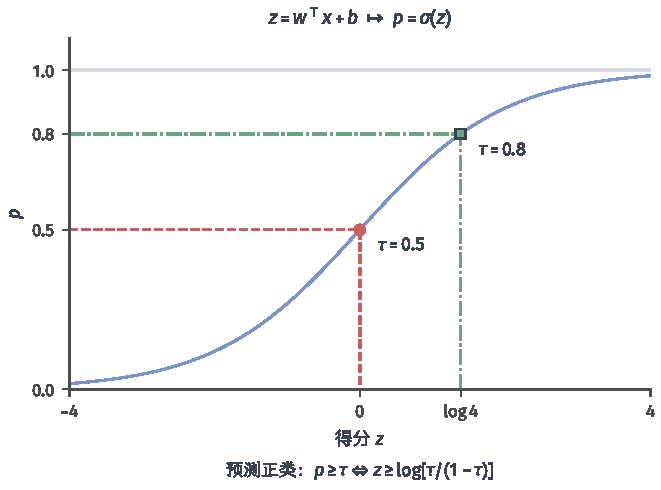
\includegraphics[width=\linewidth]{figures/03-models/01-classic-models/matplotlib/classification-logistic-probability/figure.pdf}
  \caption{线性得分$z=\bm{w}^{\top}\bm{x}+b$经Logistic函数转为正类概率$p$。蓝色实线为$p=\sigma(z)$；红色虚线与圆点标出$(0,0.5)$，绿色点划线与方点标出$(\log4,0.8)$。两组辅助线分别连接概率阈值与对应的得分阈值，数值是教学构造，不表示训练或校准结果。}
  \label{fig:classification-logistic-probability}
\end{figure}

\subsubsection{参数学习}
\label{sec:classification-logistic-learning}

对独立样本，模型给出的标签概率为$p_i^{y_i}(1-p_i)^{1-y_i}$，其中$p_i=\sigma(\bm{w}^{\top}\bm{x}_i+b)$。\term{最大似然估计}（maximum likelihood estimation, MLE）选择使已观察标签最可能出现的参数。其条件对数似然为
\begin{equation}
  \label{eq:classification-logistic-likelihood}
  \ell(\bm{w},b)
  =\sum_{i=1}^{n}
  \bigl[y_i\log p_i+(1-y_i)\log(1-p_i)\bigr].
\end{equation}
最大化$\ell$等价于最小化负对数似然$L=-\ell$，也就是二分类\term{交叉熵损失}（cross-entropy loss）：给真实标签分配的概率越低，惩罚越大。令增广输入$\tilde{\bm{x}}_i=(\bm{x}_i^{\top},1)^{\top}$、参数$\bm{\beta}=(\bm{w}^{\top},b)^{\top}\in\mathbb{R}^{d+1}$，并记$z_i=\tilde{\bm{x}}_i^{\top}\bm{\beta}$，可写成
\begin{equation}
  \label{eq:classification-logistic-loss}
  L(\bm{\beta})
  =\sum_{i=1}^{n}\bigl[\log(1+e^{z_i})-y_i z_i\bigr].
\end{equation}
数值计算不宜先求极端概率再取对数，可用$\log(1+e^z)=\max\{0,z\}+\log(1+e^{-|z|})$避免指数溢出。

为确定更新方向，利用$\sigma'(z)=\sigma(z)[1-\sigma(z)]$求导。令$\tilde{\bm{X}}\in\mathbb{R}^{n\times(d+1)}$的第$i$行为$\tilde{\bm{x}}_i^{\top}$，$\bm{p}=(p_1,\ldots,p_n)^{\top}$、$\bm{y}=(y_1,\ldots,y_n)^{\top}$，则
\begin{equation}
  \label{eq:classification-logistic-derivatives}
  \begin{aligned}
    \nabla L(\bm{\beta})
      &=\tilde{\bm{X}}^{\top}(\bm{p}-\bm{y}),\\
    \nabla^2 L(\bm{\beta})
      &=\tilde{\bm{X}}^{\top}\bm{R}\tilde{\bm{X}},\\
    \bm{R}
      &=\operatorname{diag}\bigl(p_i(1-p_i)\bigr)_{i=1}^{n}.
  \end{aligned}
\end{equation}
梯度中的$p_i-y_i$是预测概率与观察标签的差。对任意$\bm{v}\in\mathbb{R}^{d+1}$，Hessian的二次型为
\[
  \bm{v}^{\top}\nabla^2L\,\bm{v}
  =\sum_{i=1}^{n}p_i(1-p_i)
    (\tilde{\bm{x}}_i^{\top}\bm{v})^2\geq0.
\]
所以负对数似然$L$是凸函数，而被最大化的$\ell$是凹函数。有限参数处的$p_i(1-p_i)>0$；若$\tilde{\bm{X}}$列满秩，$L$严格凸，否则可能存在不改变训练得分的平坦方向。这涉及\term{可识别性}（identifiability）：数据能否区分不同参数。即使严格凸，也只能保证有限极小点若存在便唯一，不能保证它一定存在。

例如，若存在$\bm{\beta}_0$使$(2y_i-1)\tilde{\bm{x}}_i^{\top}\bm{\beta}_0>0$对所有样本成立，沿$t\bm{\beta}_0$令$t\to\infty$，每项损失均趋于零，但任意有限$t$的损失仍大于零。完全分离的数据因此没有有限MLE；准完全分离也可能使部分参数发散。完整的存在性分析区分分离、准分离和重叠情形，不能仅凭凸性断言“唯一全局最优解”\scite{albert1984existence}

实际训练常加入$\lambda\lVert\bm{w}\rVert_2^2/2$，其中$\lambda>0$。这个$L_2$惩罚抑制权重无限增大，也改善病态方向的数值条件。若两类均有样本，所有权重都受惩罚而偏置不受惩罚，所得二分类目标仍有唯一有限极小点；但若训练集只有一类，偏置仍可独自趋于无穷。若连偏置也作正的二次惩罚，则整个增广参数方向都受约束。使用$\lambda\lVert\bm{w}\rVert_1$可得到稀疏权重，但目标不再处处可微，不能直接套用下面的光滑牛顿更新。

求解器的选择取决于数据规模和存储成本。稠密数据的一轮完整梯度计算为$O(nd)$，构造Hessian约为$O(nd^2)$，直接分解又需要$O(d^3)$。若存储$d\times d$量级的Hessian过于昂贵，\term{有限内存拟牛顿法}（limited-memory BFGS, L-BFGS）只保留少量历史更新来近似二阶信息。大规模稀疏数据则可采用\term{随机梯度下降}（stochastic gradient descent, SGD），每次用一个样本或小批量近似完整梯度。选择时还应考虑稀疏程度和精度要求，而不是固定的样本数门槛。

数据持续到达时，也可以增量更新模型。McMahan等人的点击率系统使用稀疏正则与在线优化，展示了Logistic回归在大规模预测中的工程用途\scite{mcmahan2013}增量训练省去了每次从头拟合的成本，但持续更新能否改善未来预测，仍取决于更新规则和数据变化。

对于中小规模问题，\term{迭代重加权最小二乘}（iteratively reweighted least squares, IRLS）把牛顿步改写为一个权重随当前预测变化的最小二乘问题。令$\bm{J}=\operatorname{diag}(1,\ldots,1,0)$，使偏置不受惩罚。在第$t$步计算
\begin{equation}
  \label{eq:classification-logistic-irls}
  \begin{aligned}
    u_i^{(t)}
      &=z_i^{(t)}
        +\frac{y_i-p_i^{(t)}}{p_i^{(t)}(1-p_i^{(t)})},\\
    \bm{\beta}^{(t+1)}
      &\in\argmin_{\bm{\beta}}\left\{
        \begin{aligned}
          &\frac12\sum_{i=1}^{n}\bm{R}_{i,i}^{(t)}
            (u_i^{(t)}-\tilde{\bm{x}}_i^{\top}\bm{\beta})^2\\
          &\quad{}+\frac{\lambda}{2}
            \bm{\beta}^{\top}\bm{J}\bm{\beta}
        \end{aligned}
      \right\}.
  \end{aligned}
\end{equation}
这里的$u_i^{(t)}$是供当前二次近似使用的工作响应，不是新标签。对应正规方程为
\[
  \bigl(\tilde{\bm{X}}^{\top}\bm{R}^{(t)}\tilde{\bm{X}}
       +\lambda\bm{J}\bigr)\bm{\beta}^{(t+1)}
  =\tilde{\bm{X}}^{\top}\bm{R}^{(t)}\bm{u}^{(t)}.
\]
将$\bm{u}^{(t)}$代入即可还原“当前参数减去Hessian逆作用于梯度”的牛顿步。实现时应解线性方程而不显式求逆，并用阻尼或线搜索控制更新；当$p_i$接近零或一时，直接计算工作响应可能不稳定，可改用梯度与Hessian求牛顿方向。停止条件可综合梯度范数、目标变化与最大迭代次数，牛顿法的局部快速收敛不意味着从任意初始化都可无阻尼运行\scite{hastie2009}

\subsubsection{支持多分类（Softmax）}
\label{sec:classification-logistic-softmax}

新闻主题等任务要求在$C$个互斥类别中选择一个，不能把每一类都当成互不相关的二分类输出。\term{Softmax回归}（softmax regression，也称multinomial logistic regression）同时建立各类得分，并将它们转成总和为一的概率；它保留的是“任意两类的对数概率比为线性函数”这一结构。

\textbf{模型结构。}为每类引入$\bm{w}_c\in\mathbb{R}^{d}$和$b_c\in\mathbb{R}$，令$z_c(\bm{x})=\bm{w}_c^{\top}\bm{x}+b_c$。其后验模型为
\begin{equation}
  \label{eq:classification-softmax-model}
  p_c(\bm{x})
  =\mathbb{P}(y=c\mid\bm{x})
  =\frac{\exp z_c(\bm{x})}
         {\sum_{r=1}^{C}\exp z_r(\bm{x})}.
\end{equation}
指数保证概率为正，分母保证归一化；两类之间的分母相消，得到
\[
  \log\frac{p_c(\bm{x})}{p_r(\bm{x})}
  =(\bm{w}_c-\bm{w}_r)^{\top}\bm{x}+b_c-b_r.
\]
当$C=2$时，$p_1(\bm{x})=\sigma((\bm{w}_1-\bm{w}_2)^{\top}\bm{x}+b_1-b_2)$。把第1类视为正类、第2类视为负类，就回到二分类Logistic回归。

共同增加得分不会改变概率。更具体地，对任意$\bm{a}\in\mathbb{R}^{d}$和$t\in\mathbb{R}$，变换$\bm{w}_c\mapsto\bm{w}_c+\bm{a}$、$b_c\mapsto b_c+t$使每个指数项同乘$\exp(\bm{a}^{\top}\bm{x}+t)$，因而全部约掉。这是$d+1$维的参数冗余。选择第$C$类为\term{参考类}（reference class），就是把该类完整的增广参数固定为零：
\begin{equation}
  \label{eq:classification-softmax-reference}
  \begin{gathered}
    \bm{w}_C=\bm{0},\qquad b_C=0,\\
    \log\frac{p_c(\bm{x})}{p_C(\bm{x})}
    =\bm{w}_c^{\top}\bm{x}+b_c
    \quad(c<C).
  \end{gathered}
\end{equation}
仅固定$\bm{w}_C$而不固定$b_C$不够。类似地，$\lambda\sum_c\lVert\bm{w}_c\rVert_2^2/2$能够消除共同权重平移的自由，却不能锁定共同偏置平移；仍须约束偏置，例如令$\sum_c b_c=0$，或惩罚全部偏置。消除这种固有冗余后，还应检查训练设计矩阵的秩与数据分离，不能把这些不同问题混为一谈。

\textbf{参数学习。}现在$y_i\in\{1,\ldots,C\}$，记$p_{i,c}=p_c(\bm{x}_i)$，$\bm{\Theta}\in\mathbb{R}^{(d+1)\times C}$的第$c$列为$\bm{\beta}_c=(\bm{w}_c^{\top},b_c)^{\top}$。多类负对数似然是
\begin{equation}
  \label{eq:classification-softmax-loss}
  \begin{aligned}
    L(\bm{\Theta})
      &=-\sum_{i=1}^{n}\log p_{i,y_i}\\
      &=\sum_{i=1}^{n}\left[
        \log\sum_{c=1}^{C}e^{z_c(\bm{x}_i)}
        -z_{y_i}(\bm{x}_i)\right].
  \end{aligned}
\end{equation}
以$\mathbb{1}\{\cdot\}$表示条件成立时为一、否则为零的指示函数，梯度为
\begin{equation}
  \label{eq:classification-softmax-gradient}
  \begin{aligned}
    \nabla_{\bm{w}_c}L
      &=\sum_{i=1}^{n}
        [p_{i,c}-\mathbb{1}\{y_i=c\}]\bm{x}_i,\\
    \frac{\partial L}{\partial b_c}
      &=\sum_{i=1}^{n}
        [p_{i,c}-\mathbb{1}\{y_i=c\}].
  \end{aligned}
\end{equation}
它仍由“预测减观察”的残差驱动。Hessian的$(c,r)$参数块为
\[
  \nabla^2_{\bm{\beta}_c,\bm{\beta}_r}L
  =\sum_{i=1}^{n}p_{i,c}
    [\mathbb{1}\{c=r\}-p_{i,r}]
    \tilde{\bm{x}}_i\tilde{\bm{x}}_i^{\top}.
\]
对任意增广参数扰动$\bm{v}_c$，令$a_{i,c}=\tilde{\bm{x}}_i^{\top}\bm{v}_c$，相应二次型为
\[
  \sum_{i=1}^{n}\left[
    \sum_{c=1}^{C}p_{i,c}a_{i,c}^2
    -\left(\sum_{c=1}^{C}p_{i,c}a_{i,c}\right)^2
  \right]\geq0.
\]
方括号正是以$\bm{p}_i$为权重的方差，故$L$凸。共同平移使方差为零，秩亏还会引入其他平坦方向；分离数据上同样可能不存在有限MLE。参考类约束解决表示冗余，适当正则化控制参数大小，两者的作用不同。

Softmax可用分块牛顿法、L-BFGS或小批量SGD优化，多类Hessian还包含类别间的耦合，不能简单把$C$个独立的二分类IRLS问题拼起来。求概率时应先减去$m(\bm{x})=\max_c z_c(\bm{x})$，用$e^{z_c-m}/\sum_r e^{z_r-m}$得到完全相同且更稳定的结果。普通稠密实现的一轮梯度计算约为$O(ndC)$。

类别特别多时，分母求和也会成为瓶颈。\term{层次Softmax}（hierarchical softmax）以树上路径概率的乘积替代平坦分类参数化；\term{噪声对比估计}（noise-contrastive estimation, NCE）通过区分数据与人为噪声来估计模型；\term{负采样}（negative sampling）只对抽取的负例建立局部区分目标。三者都可减少某些计算，但不能统称为原Softmax似然的等价计算，尤其负采样通常改变了训练目标\scite{goodfellow2016}

\textbf{决策与概率语义。}预测可取$\hat y(\bm{x})=\argmax_c p_c(\bm{x})=\argmax_c z_c(\bm{x})$，并按固定类别次序处理平局。Softmax输出已经满足概率公理，却不自动满足\term{概率校准}（probability calibration）：在被预测为某类概率约为$0.8$的样本中，该类的实际比例也应接近$0.8$。有限样本、模型失配、正则化和分布变化都可能破坏这种对应。

Softmax常用作神经网络的分类输出层，但其归一化也不能保证整个网络校准。Guo等对现代网络的实验表明，分类准确与置信度可靠可以明显分离；独立验证数据上的温度缩放等方法能改善一些设置下的校准，却仍不是任意新分布下的保证\scite{guo2017calibration}

\subsubsection{小结}
\label{sec:classification-logistic-summary}

Logistic回归把线性得分、条件概率与代价敏感阈值连接起来，多类版本则用Softmax联合比较各类。固定特征表示下的训练目标凸，便于优化与复核；权重也可在对数几率尺度上解释。但可识别性、有限解的存在性和概率校准分别需要检查，不能从“凸目标”或“概率输出”一并推出。

它的表示限制来自线性对数几率：若需要非线性交互，应显式加入交叉项或其他特征变换。训练可通过随机优化增量进行，预测则只需保存参数并计算得分。信用评分、医学风险预测和点击率预估都可以采用这种基线，但具体特征与验证方式需要对应到各自任务。

\subsection{朴素贝叶斯}
\label{sec:classification-naive-bayes}

若希望通过“哪一类更可能产生当前输入”来分类，就需要估计类条件分布。困难在于，$d$个二值特征已有$2^d$种组合，逐一统计需要大量样本。\term{朴素贝叶斯}（naive Bayes, NB）把复杂的联合分布拆成较小的分布，用简化假设换取少量统计量和直接的参数估计。这样的约束可能降低有限样本下的估计波动，也可能引入持续的模型偏差，并不无条件提高精度。

Maron在1961年关于自动索引的研究，是概率方法用于文档归类的早期工作之一。文档分类需要从大量词项中提取可累积的类别证据，这也成为朴素贝叶斯的一项典型用途\scite{maron1961indexing}

\subsubsection{模型结构}
\label{sec:classification-naive-bayes-structure}

对一般特征向量，NB采用给定类别后的\term{条件独立}（conditional independence）假设：已知$y=c$后，一个特征的取值不再改变其他特征的分布。令$\pi_c=\mathbb{P}(y=c)$、$p_{j,c}(x_j)=p(x_j\mid y=c)$，模型写成
\begin{equation}
  \label{eq:classification-naive-bayes-model}
  \begin{aligned}
    q_c(\bm{x})&=\prod_{j=1}^{d}p_{j,c}(x_j),\\
    \mathbb{P}_{\mathrm{NB}}(y=c\mid\bm{x})
      &=\frac{\pi_c q_c(\bm{x})}
      {\sum_{r=1}^{C}\pi_r q_r(\bm{x})}.
  \end{aligned}
\end{equation}
记号$q_c$强调这是模型使用的乘积分布，未必等于真实类条件分布。条件独立不要求全部训练样本混在一起时特征仍独立，例如词项之间的总体相关性可能部分来自主题差异。

只需要分类时，各类共同的分母可以省略。为避免许多小概率连乘下溢，通常比较对数得分
\begin{equation}
  \label{eq:classification-naive-bayes-score}
  s_c(\bm{x})
  =\log\pi_c+\sum_{j=1}^{d}\log p_{j,c}(x_j),
  \qquad
  \hat y(\bm{x})=\argmax_c s_c(\bm{x}).
\end{equation}
这里$s_c$不是归一化的对数后验；需要概率时还须减去$\log\sum_r e^{s_r}$。零概率可使得分为负无穷，后面的平滑正是为未见事件保留概率质量。文档的多项式版本沿用相似得分，但它的独立性对象是词元位置，而非总长度固定后的各维计数，必须另外说明。

\subsubsection{参数学习}
\label{sec:classification-naive-bayes-learning}

令$n_c=\sum_i\mathbb{1}\{y_i=c\}$，类先验的MLE为$\hat\pi_c=n_c/n$。这是以训练样本的类别比例估计目标总体的比例，依赖抽样具有代表性；若训练集人为重采样，不能未经修正就把重采样后的比例当成部署先验。也可以使用有依据的外部类别比例；若希望保留对该比例的不确定性，并为训练中未见的类别保留概率质量，则可对类概率向量$\bm{\pi}=(\pi_1,\ldots,\pi_C)^{\top}$设置参数先验。以下对类别概率与各组类条件参数设置相互独立的先验，以便分别更新。

使用\BookSectionRef{sec:probability-common-distributions}{第一卷“数学准备”的常见分布模型小节}
中的\term{Dirichlet分布}，给类概率向量设置正参数$\gamma_c$的先验。
独立类别记录的计数进入各坐标的幂次，因而
\[
  \begin{aligned}
    p(\bm{\pi})
      &\propto\prod_{c=1}^{C}\pi_c^{\gamma_c-1},\\
    p(y_1,\ldots,y_n\mid\bm{\pi})
      &\propto\prod_{c=1}^{C}\pi_c^{n_c},\\
    p(\bm{\pi}\mid y_1,\ldots,y_n)
      &\propto\prod_{c=1}^{C}\pi_c^{\gamma_c+n_c-1}.
  \end{aligned}
\]
后验仍是Dirichlet分布，只需把参数从$\gamma_c$更新为$\gamma_c+n_c$。
这种先验与后验属于同一分布族的关系称为\term{共轭}（conjugacy）。
使用卷一的均值公式，后验均值为
\[
  \tilde\pi_c=\frac{n_c+\gamma_c}
  {n+\sum_{r=1}^{C}\gamma_r}.
\]
先验均值为$\gamma_c/\sum_r\gamma_r$，参数总和决定这些伪计数相对于观测计数的权重。这里“类别先验$\pi_c$”是样本生成模型的一部分，“参数先验”则表达估计$\bm{\pi}$前的不确定性，两者不是同一个概率。

连续特征可采用\term{高斯朴素贝叶斯}（Gaussian naive Bayes），即$x_j\mid y=c\sim\mathcal{N}(\mu_{j,c},\sigma_{j,c}^{2})$，其中$\sigma_{j,c}^{2}>0$。当$n_c>0$且该特征的类内平方偏差和为正时，均值和方差的MLE为
\begin{equation}
  \label{eq:classification-naive-bayes-gaussian}
  \begin{aligned}
    \hat\mu_{j,c}
      &=\frac{1}{n_c}\sum_{i:y_i=c}x_{i,j},\\
    \hat\sigma_{j,c}^{2}
      &=\frac{1}{n_c}\sum_{i:y_i=c}
        (x_{i,j}-\hat\mu_{j,c})^2.
  \end{aligned}
\end{equation}
方差分母为$n_c$，不是无偏样本方差所用的$n_c-1$。在上述条件下，预测时将这些量代入一维高斯密度后相乘。若某类某特征恒定为$a$，固定$\mu_{j,c}=a$后，对数似然为$-n_c\log(2\pi\sigma_{j,c}^{2})/2$，随正方差趋于零而无界增大。因此，此时正方差参数域内没有有限MLE；式\eqref{eq:classification-naive-bayes-gaussian}给出的零值只是样本散度，不能代入普通高斯密度。设定有明确尺度的方差下限或加入先验后，得到的是相应的受约束或正则化估计；给密度任意“加一”不是离散概率的平滑对应物。

只关心某个词是否出现时，可用\term{伯努利朴素贝叶斯}（Bernoulli naive Bayes）。输入$x_{i,j}\in\{0,1\}$，令$n_{j,c}=\sum_{i:y_i=c}x_{i,j}$，则
\begin{equation}
  \label{eq:classification-naive-bayes-bernoulli}
  \begin{aligned}
    q_c(\bm{x})
      &=\prod_{j=1}^{d}
        \theta_{j,c}^{x_j}(1-\theta_{j,c})^{1-x_j},\\
    \hat\theta_{j,c}&=\frac{n_{j,c}}{n_c}.
  \end{aligned}
\end{equation}
未出现的词同样提供证据，不能只保留$x_j=1$的项；这里的MLE要求$n_c>0$。
为平滑这个二值事件，使用卷一的Beta分布作为$\theta_{j,c}$的先验，
两个正参数$\alpha_1,\alpha_0$分别对应出现与未出现。乘以似然后，
两项指数分别增加$n_{j,c}$和$n_c-n_{j,c}$，所以
\[
  \theta_{j,c}\mid D_n
  \sim\operatorname{Beta}
    (\alpha_1+n_{j,c},\,\alpha_0+n_c-n_{j,c}).
\]
其后验均值为$(n_{j,c}+\alpha_1)/(n_c+\alpha_1+\alpha_0)$；对称情形$\alpha_1=\alpha_0=\alpha$的分母是$n_c+2\alpha$。这同时平滑了出现和未出现两种事件。

若重复出现的次数也有意义，应使用\term{多项式朴素贝叶斯}（multinomial naive Bayes）。设固定词表有$d$个词项，$\bm{x}_i\in\mathbb{N}_0^d$记录一篇文档的词项计数，$m_i=\sum_jx_{i,j}$是该文档的总词元数。给定类别和$m_i$，假设每个词元位置独立地按$\bm{\theta}_c=(\theta_{1,c},\ldots,\theta_{d,c})^{\top}$抽取词项，其中$\sum_j\theta_{j,c}=1$。忽略顺序后，计数向量服从
\begin{equation}
  \label{eq:classification-naive-bayes-multinomial}
  \mathbb{P}(\bm{x}_i\mid y_i=c,m_i)
  =\frac{m_i!}{\prod_{j=1}^{d}x_{i,j}!}
    \prod_{j=1}^{d}\theta_{j,c}^{x_{i,j}}.
\end{equation}
因为计数总和已固定，各维计数并不独立。将它写成每维整数取值的独立类别分布，会改变模型和分母。McCallum与Nigam专门比较了伯努利和多项式这两种文档事件模型，明确区分“词是否出现”与“词出现多少次”\scite{mccallum1998event}

标准文档分类通常进一步假设长度分布与类别无关，因而$\mathbb{P}(m_i\mid y_i=c)$在类别比较中约掉，此时给定长度后的类先验仍为$\pi_c$。若长度本身携带类别信息，则应保留并估计该项，使长度也参与后验计算。

令$t_{j,c}=\sum_{i:y_i=c}x_{i,j}$为第$c$类中词项$j$的总出现次数，$t_c=\sum_jt_{j,c}$为该类的总词元数。去掉与参数无关的组合系数后，类内对数似然为$\sum_jt_{j,c}\log\theta_{j,c}$。当$t_c>0$时，在$\sum_j\theta_{j,c}=1$约束下求极值，正计数坐标上的拉格朗日方程给出$t_{j,c}/\theta_{j,c}$为同一常数，零计数坐标取零；求和确定常数为$t_c$，从而得到频率MLE。

若对$\bm{\theta}_c$使用$\operatorname{Dirichlet}(\alpha_1,\ldots,\alpha_d)$先验，其中$\alpha_j>0$，同样的共轭更新把各坐标的幂次从$\alpha_j-1$变为$\alpha_j+t_{j,c}-1$，得到
\[
  \bm{\theta}_c\mid D_n
  \sim\operatorname{Dirichlet}
    (\alpha_1+t_{1,c},\ldots,\alpha_d+t_{d,c}).
\]
把更新后的参数归一化即可得到后验均值。两种估计分别为
\begin{equation}
  \label{eq:classification-naive-bayes-smoothing}
  \hat\theta_{j,c}=\frac{t_{j,c}}{t_c},
  \qquad
  \tilde\theta_{j,c}
  =\frac{t_{j,c}+\alpha_j}
         {t_c+\sum_{r=1}^{d}\alpha_r}.
\end{equation}
前式要求$t_c>0$；后式也给出下一词元的后验预测概率，因为给定参数时该概率为$\theta_{j,c}$，对参数后验积分便得到其后验均值。这种均值估计通常既不同于MLE，也不同于式\eqref{eq:regression-map}定义的MAP。对称$\alpha_j=1$给出\term{拉普拉斯平滑}（Laplace smoothing），相当于每个词项加入一个伪计数；$\alpha_j=1/2$对应多项式参数的Jeffreys先验。对伯努利参数，其对应物是$\operatorname{Beta}(1/2,1/2)$，不应把这些常数不加区分地推广到高斯方差。以平滑估计代入式\eqref{eq:classification-naive-bayes-multinomial}得到的是常用的点估计分类器，不等于积分消去参数后的整篇文档预测分布。

在长度与类别无关的约定下，文档预测只需计算$\log\tilde\pi_c+\sum_jx_j\log\tilde\theta_{j,c}$。算法\ref{alg:classification-multinomial-nb}给出完整的统计与预测流程，训练和预测使用相同的词表，并明确处理平滑与得分平局。
\begin{algorithm}[带平滑的多项式朴素贝叶斯]
  \label{alg:classification-multinomial-nb}
  \begin{algorithmic}[1]
    \Require 非空训练集$D_n$，固定词表大小$d$与类别数$C$；
    \Statex \hspace{\algorithmicindent} 词项伪计数$\alpha>0$，类别伪计数$\gamma>0$
    \Ensure 类先验$\tilde{\bm{\pi}}$、词项概率$\tilde{\bm{\Theta}}$及预测规则
    \State 检查所有输入为有限非负整数计数，标签属于$\{1,\ldots,C\}$
    \State 将$n_c$、$t_c$与$t_{j,c}$全部初始化为零
    \For{$i=1,\ldots,n$}
      \State 令$c=y_i$，并更新$n_c\gets n_c+1$
      \For{满足$x_{i,j}>0$的词项$j$}
        \State $t_{j,c}\gets t_{j,c}+x_{i,j}$
        \State $t_c\gets t_c+x_{i,j}$
      \EndFor
    \EndFor
    \For{$c=1,\ldots,C$}
      \State $\tilde\pi_c\gets(n_c+\gamma)/(n+C\gamma)$
      \State 对所有$j$，令$\tilde\theta_{j,c}\gets(t_{j,c}+\alpha)/(t_c+d\alpha)$
    \EndFor
    \State 对新计数向量$\bm{x}$，按相同词表与输入检查计算
    \Statex \hspace{\algorithmicindent}
      $s_c=\log\tilde\pi_c+\sum_{j:x_j>0}x_j\log\tilde\theta_{j,c}$
    \State 返回$s_c$最大的类别；平局时返回索引最小的类别
  \end{algorithmic}
\end{algorithm}

假设词表只有三个词项，两类累计计数分别为$(3,1,0)$和$(0,1,3)$，类先验均为$1/2$。取$\alpha=1$，平滑后的词项概率分别为$(4,2,1)/7$和$(1,2,4)/7$。对新文档$\bm{x}=(1,0,1)^{\top}$，两类乘积相同，判决平局；对$\bm{x}=(2,0,1)^{\top}$，两类得分之差为$\log4$，于是选择第1类。这个教学例子显示了重复计数怎样改变证据，而零计数词项经平滑后不会把整类概率直接清零。

\subsubsection{理论分析}
\label{sec:classification-naive-bayes-theory}

\paragraph{收敛性分析}
NB的计数估计有闭式表达式，这里的收敛问题不是迭代优化何时停止，而是样本增加后估计量趋向什么。固定特征维数、类别数和有限取值集合，在独立同分布抽样且各类先验为正时，强大数定律保证经验类频率和类内相对频率几乎必然收敛到对应的真实概率。固定伪计数相对于不断增长的类内样本数趋于零，因此不改变这一极限。

单维条件概率估计一致，并不要求同一样本的各维特征条件独立；但把这些概率相乘后能否还原真实联合分布，需要额外的模型假设。高斯NB若要一致地估计类条件密度，还要求高斯族正确、方差非退化并使用一致估计。多项式NB则要求词元生成与长度处理假设正确，训练文档的抽样及总计数满足相应大数定律。有限离散情形的频率收敛证明包含在下面的风险一致性证明中。

\paragraph{泛化分析}
估计量收敛后，还需回答由这些估计构造的分类器能否接近贝叶斯风险。下面先在模型正确的有限离散情形下给出完整证明，再考察条件独立不成立时，哪些依赖会改变决策。这个结论描述样本数趋于无穷时的风险，不是有限样本的误差上界，也无需排除后验平局。
\begin{theorem}[有限离散特征下NB的风险一致性]
  \label{thm:classification-naive-bayes-consistency}
  设$d$、$C$固定，每维特征的取值集合有限，训练样本独立同分布，且每类先验$\pi_c>0$。若真实分布满足给定类别后的特征条件独立，使用经验类频率与类内相对频率估计概率，或加入固定的正伪计数，则所得NB分类器$\hat h_n$满足
  \[
    R(\hat h_n)\longrightarrow R^\ast
    \quad\text{几乎必然}.
  \]
  这里$R(h)=\mathbb{P}(h(\bm{X})\neq Y)$针对独立的新样本计算，$R^\ast$为贝叶斯风险；几乎必然收敛针对无限训练样本序列。早期若$n_c=0$，可任意指定该类的条件分布；若某输入的全部类别得分为零，也可任意指定该处的预测。
\end{theorem}
\begin{proof}
  对取值$v$及$n_c>0$的类别，类内估计为
  \[
    \hat p_{j,c}(v)
    =\frac{\sum_{i=1}^{n}\mathbb{1}\{x_{i,j}=v,y_i=c\}}
           {n_c}.
  \]
  由强大数定律，$n_c/n\to\pi_c>0$，故空类别事件几乎必然最终不再出现。分子除以$n$收敛到$\mathbb{P}(X_j=v,Y=c)$，因此$\hat p_{j,c}(v)\to p_{j,c}(v)$几乎必然。固定伪计数相对于$n_c$趋于零，不改变极限。有限多个估计可同时收敛；对每个$\mathbb{P}(\bm{X}=\bm{x})>0$的输入，归一化分母最终为正，早期任意约定不影响极限。乘积与归一化于是给出
  \[
    \hat\eta_{n,c}(\bm{x})
    \longrightarrow
    \eta_c(\bm{x})=\mathbb{P}(Y=c\mid\bm{X}=\bm{x}).
  \]
  令$c^\ast$最大化真实后验，$\hat c$最大化估计后验。因为$\hat\eta_{n,\hat c}\geq\hat\eta_{n,c^\ast}$，插入这两个估计值得到
  \[
    0\leq\eta_{c^\ast}(\bm{x})-\eta_{\hat c}(\bm{x})
    \leq2\max_c|\hat\eta_{n,c}(\bm{x})-\eta_c(\bm{x})|.
  \]
  左侧就是该输入处的超额分类风险。对有限个输入按真实概率加权求和，右侧趋于零，故整体风险趋于$R^\ast$。
\end{proof}

后验平局时，最大化类别可能随$n$变化，但选择不同的最优类别并不增加风险。因此，风险一致性不等于决策最终处处固定，更不能由“依概率收敛”直接推出无条件的决策几乎必然一致。若模型失配，估计可能稳定地收敛到不同于真实联合分布的乘积分布；增加样本能减小估计误差，却不会自动消除这种模型偏差。

真实数据中的词语、测量量和相邻像素常有依赖，但违反独立性并不直接决定分类误差。Domingos与Pazzani在1997年的研究区分了概率估计误差与零一分类损失，报告了含依赖数据上的经验结果，并在特定条件下分析了合取、析取概念等情形的最优性。分类只要求最高得分类别正确，因此概率估计失真与分类仍然准确可以同时发生\scite{domingos1997optimality}

为拆开这些层次，暂取二分类$c\in\{0,1\}$，并使用真实类先验与真实单维条件分布构造总体NB，不含有限样本估计误差。在下列分母均为正的输入处，定义
\begin{equation}
  \label{eq:classification-naive-bayes-ratios}
  \begin{aligned}
    r(\bm{x})
      &=\frac{\pi_1p(\bm{x}\mid y=1)}
              {\pi_0p(\bm{x}\mid y=0)},\\
    r_{\mathrm{NB}}(\bm{x})
      &=\frac{\pi_1\prod_jp(x_j\mid y=1)}
              {\pi_0\prod_jp(x_j\mid y=0)}.
  \end{aligned}
\end{equation}
若平局都归第1类，则两个分类器在该输入上的决策相同，当且仅当$r\geq1$与$r_{\mathrm{NB}}\geq1$同真同假。理由只是：用正的第0类联合得分除两边，不改变类别得分的大小关系。这是从判决规则直接得到的等价关系，不是对NB有效范围的独立保证；其中$r$还是未知真分布的量。

要解释依赖何时不会改变比值，可以进一步定义
\begin{equation}
  \label{eq:classification-naive-bayes-dependence}
  \begin{aligned}
    a_c(\bm{x})
      &=\frac{p(\bm{x}\mid y=c)}
              {\prod_{j=1}^{d}p(x_j\mid y=c)},\\
    r(\bm{x})
      &=r_{\mathrm{NB}}(\bm{x})
        \frac{a_1(\bm{x})}{a_0(\bm{x})}.
  \end{aligned}
\end{equation}
$a_c$衡量真实联合分布相对于乘积分布的修正。条件独立使$a_c=1$；更弱的充分条件是$a_1=a_0>0$，此时即使两类内部都有依赖，其修正在类别比值中也完全相消。由概率链式法则还可写成
\[
  a_c(\bm{x})
  =\prod_{j=1}^{d}
    \frac{p(x_j\mid x_1,\ldots,x_{j-1},y=c)}
         {p(x_j\mid y=c)}.
\]
各因子不必分别为一，不同位置的修正也可在整体乘积中抵消。所需比较的是两类中这些概率修正的比值，而不只是通常的相关系数。Zhang在2004年以局部依赖比和全局依赖分布因子展开了这一思路\scite{zhang2004optimality}

完全相消仍只是充分条件。若$r_{\mathrm{NB}}\neq1$，且
\[
  \left|\log a_1(\bm{x})-\log a_0(\bm{x})\right|
  <\left|\log r_{\mathrm{NB}}(\bm{x})\right|,
\]
则修正不足以改变对数比的正负，决策仍然相同。反之，依赖影响在两类中不均衡时就可能越过边界。例如把一个有信息的二值特征原样复制一次，在等类先验下，NB把原似然比平方：原比值为4时，真实后验为$4/5$，NB却报$16/17$，分类未变而置信度偏高。非等先验下，特征证据被重复计算还可能改变类别，这说明同一个依赖错误对概率与决策的影响可以不同。

\subsubsection{小结}
\label{sec:classification-naive-bayes-summary}

NB的计算优势来自统计量可累积：稠密输入的训练统计约为$O(nd)$，存储为$O(Cd)$，单样本预测为$O(Cd)$，这些量级以每维分布的参数个数有界为前提。以$\bm{X}\in\mathbb{R}^{n\times d}$记训练输入矩阵，多项式模型可按非零计数累积，训练约为$O(n+\operatorname{nnz}(\bm{X})+Cd)$，预测约为$O(C(1+\operatorname{nnz}(\bm{x})))$。这里$\operatorname{nnz}$表示非零元素数；“扫描一次”不意味着与样本数、特征数和类别数都无关。

它适合建立文档、垃圾邮件和情感分类的低成本基线，也容易增量更新。Graham在2002年8月的《A Plan for Spam》中介绍了基于词项统计的邮件过滤实践；该方法还加入词项筛选与经验修正，与本节的标准多项式模型有所不同\scite{graham2002spam}

使用NB时要分别检查输入的事件模型、特征依赖和概率校准。相关性可能造成证据重复计算，却不必然破坏分类；连续特征还可能因所选单维分布失配而出错。若业务需要可靠概率，应另用留出数据评估和校准，而不只报告准确率。

\subsection{高斯判别分析（GDA）}
\label{sec:classification-gda}

高斯NB只保存每维的均值与方差，相当于把类内协方差矩阵的非对角元素设为零。若分类信息恰好体现在多个连续特征的共同变化中，就需要估计这些关系。\term{高斯判别分析}（Gaussian discriminant analysis, GDA）用每类的多元高斯分布描述输入，允许保留类内协方差；增加的表达能力也意味着需要估计更多参数。

第\ref{sec:clustering-gmm}节的高斯混合模型同样估计高斯成分及其权重，但成分归属是潜变量，通常用\term{期望最大化}（expectation-maximization, EM）交替计算成分归属的后验概率并更新分布参数；两步计算的分类实例见第\ref{sec:classification-semisupervised-comparison}节。GDA中的类别标签已经观测，可以直接按类分组估计。两者共享高斯密度结构，却分别服务于预设类别预测和无标签分组。

从类间分离程度转向概率决策，关注的问题也从“怎样区分类别”扩展为“怎样权衡误判”。Anderson在1951年的多元分类研究中，以误分类代价为依据讨论分类规则，并在正态总体下给出判别函数。这为理解GDA提供了一条历史线索：分布模型负责描述输入来自各类的可能性，决策规则再据此比较误判代价，而不只是寻找一个投影方向\scite{anderson1951classification}

\subsubsection{模型结构}
\label{sec:classification-gda-structure}

本节用GDA统称各类具有高斯条件分布的判别模型，并分别讨论共享协方差与类特有协方差。对第$c$类，参数是$\pi_c$、$\bm{\mu}_c\in\mathbb{R}^{d}$及对称正定的$\bm{\Sigma}_c\in\mathbb{R}^{d\times d}$：
\begin{equation}
  \label{eq:classification-gda-density}
  \begin{aligned}
    p(\bm{x}\mid y=c)
      &=\frac{\exp[-\Delta_c(\bm{x})/2]}
        {(2\pi)^{d/2}|\bm{\Sigma}_c|^{1/2}},\\
    \Delta_c(\bm{x})
      &=(\bm{x}-\bm{\mu}_c)^{\top}
        \bm{\Sigma}_c^{-1}(\bm{x}-\bm{\mu}_c).
  \end{aligned}
\end{equation}
这里的二次型$\Delta_c$按类内变化尺度衡量输入偏离均值的程度；行列式项则补偿分布体积，不能在不同协方差的类别比较中丢掉。贝叶斯后验仍为$\pi_cp(\bm{x}\mid y=c)/\sum_r\pi_rp(\bm{x}\mid y=r)$。

取对数并删除所有类别共有的$-d\log(2\pi)/2$，得到判别得分
\begin{equation}
  \label{eq:classification-gda-score}
  g_c(\bm{x})
  =\log\pi_c-\frac12\log|\bm{\Sigma}_c|
   -\frac12\Delta_c(\bm{x}).
\end{equation}
预测选择最大$g_c$。这一模型不要求各特征独立，但要求整类分布可由单个多元高斯刻画；“保留完整协方差”只是保留全部二阶关系，不是能表达任意非线性依赖或多峰结构。

\subsubsection{参数学习}
\label{sec:classification-gda-learning}

有标签时，各类样本的归属已知，联合对数似然可按类别分开优化。当每类都有样本且类内散度矩阵正定时，MLE为
\begin{equation}
  \label{eq:classification-gda-estimates}
  \begin{aligned}
    \hat\pi_c&=\frac{n_c}{n},\\
    \hat{\bm{\mu}}_c
      &=\frac{1}{n_c}\sum_{i:y_i=c}\bm{x}_i,\\
    \hat{\bm{\Sigma}}_c
      &=\frac{1}{n_c}\sum_{i:y_i=c}
        (\bm{x}_i-\hat{\bm{\mu}}_c)
        (\bm{x}_i-\hat{\bm{\mu}}_c)^{\top}.
  \end{aligned}
\end{equation}
均值来自使类内平方偏差最小的驻点，协方差来自似然中的对数行列式与二次型之间的平衡。和高斯NB一样，这里使用MLE分母$n_c$；若改用$n_c-1$，得到的是无偏协方差估计。若类内散度奇异，沿未被样本覆盖的方向收缩方差可使似然不断增大，在协方差正定的参数域内没有有限MLE；此时上式的奇异矩阵只能作为样本散度统计，不能当成合法的普通高斯协方差。

共享协方差特例的完整推导已经放在第\ref{sec:classification-lda}节。简要地说，约束$\bm{\Sigma}_c=\bm{\Sigma}$后，合并类内散度给出式~\eqref{eq:classification-lda-covariance}~的MLE；展开高斯得分时，各类共有的$\bm{x}^{\top}\bm{\Sigma}^{-1}\bm{x}$相消，得到式~\eqref{eq:classification-lda-score}~的线性得分。两类得分相等因而给出超平面。若协方差随类变化，二次项一般不能约掉，得到QDA及通常为二次曲面的两类边界。共享与否改变的不是贝叶斯规则，而是允许的分布族及由此得到的得分形式\scite{bishop2006}

图\ref{fig:classification-gaussian-boundaries}在同一个二维教学例子中比较两种协方差设定。两图都取$\pi_1=\pi_2=1/2$、$\bm{\mu}_1=(-1,0)^{\top}$、$\bm{\mu}_2=(1,0)^{\top}$，坐标为无量纲特征。左图共享$\bm{\Sigma}_1=\bm{\Sigma}_2=\bm{I}_2$；右图只将第2类改为$\bm{\Sigma}_2=\operatorname{diag}(1,4)$。代入式\eqref{eq:classification-gda-score}，得分差分别为
\begin{equation}
  \label{eq:classification-gda-boundary-example}
  \begin{aligned}
    g_2-g_1&=2x_1
      &&\text{（共享协方差）},\\
    g_2-g_1&=2x_1+\frac38x_2^2-\log2
      &&\text{（类特有协方差）}.
  \end{aligned}
\end{equation}
令得分差为零，得到直线$x_1=0$和抛物线$x_1=\frac12\log2-\frac{3}{16}x_2^2$。在两种设定中，边界右侧的$g_2$都更大，预测第2类。右图中，第2类沿$x_2$方向更分散：在$x_2=0$附近，行列式项降低了它的密度峰值，边界向右移到$x_1\approx0.347$；随着$|x_2|$增大，第2类较慢衰减的密度又使其预测区域向左延伸。只看均值之间的距离，会漏掉方差尺度和密度归一化对判决的共同影响。
\begin{figure*}[htbp]
  \centering
  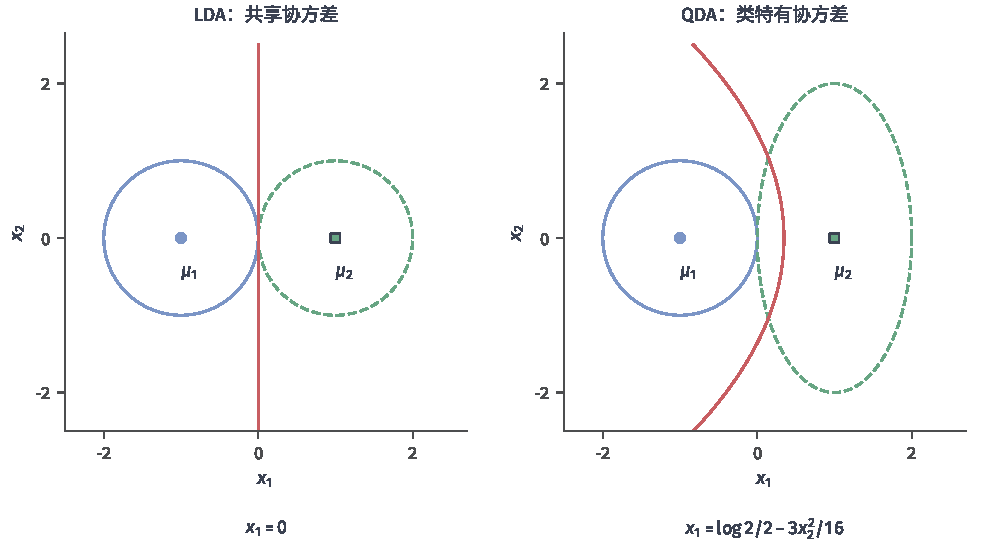
\includegraphics[width=\linewidth]{figures/03-models/01-classic-models/matplotlib/classification-gaussian-boundaries/figure.pdf}
  \caption{两图均取$\pi_1=\pi_2=1/2$、$\bm{\mu}_1=(-1,0)^{\top}$、$\bm{\mu}_2=(1,0)^{\top}$和$\bm{\Sigma}_1=\bm{I}_2$，仅第2类协方差变化。蓝色圆点和绿色方点为均值，蓝色实线与绿色虚线分别为$\Delta_1=1$和$\Delta_2=1$的等密度轮廓；不同类的这些轮廓不保证密度值相同。红色粗线按$g_1=g_2$的解析式绘制，底部公式分别给出LDA的线性边界与QDA的二次边界。参数均为教学构造，不是采样或拟合结果。}
  \label{fig:classification-gaussian-boundaries}
\end{figure*}

对二分类，把式~\eqref{eq:classification-lda-score}~中的两类得分相减并归一化，就得到Logistic形式的后验。因此，共享高斯假设蕴含线性对数几率，反过来却不成立；许多非高斯输入分布也能有Logistic形式的条件概率。即便两条路线的后验形式相同，用联合似然估计均值和协方差，与直接最大化条件似然，也通常得到不同的有限样本参数。

完整协方差每类需要$d(d+1)/2$个自由参数。类内散布矩阵的秩至多为$n_c-1$，因而$n_c\leq d$时必然奇异，不能直接代入普通高斯密度；$n_c>d$也不保证估计准确或条件良好。共享估计的秩至多为$n-C$。在维数较大或类别样本少时，可以共享、取对角，或采用
\[
  \tilde{\bm{\Sigma}}_c
  =(1-\rho)\hat{\bm{\Sigma}}_c+\rho\tau\bm{I}_d,
  \qquad 0<\rho\leq1,\quad\tau>0
\]
这样的收缩估计。$\tau$提供方差尺度，$\rho$控制偏离样本协方差的程度；这是改变估计准则，不再是未经约束的MLE。

稠密完整协方差的统计成本约为$O(nd^2)$，各类矩阵分解约为$O(Cd^3)$，存储为$O(Cd^2)$，QDA单样本得分约为$O(Cd^2)$。LDA只需分解一份协方差，并可预先算出线性权重，使单样本预测降到$O(Cd)$。实现时可用Cholesky分解求解二次型与对数行列式，无须显式构造逆矩阵。

\subsubsection{小结}
\label{sec:classification-gda-summary}

GDA用同一套生成式模型连接高斯NB、LDA与QDA：对角协方差忽略类内相关，共享协方差降低估计负担，类特有完整协方差则允许更灵活的边界。三者的选择要结合每类样本量、维数和类内结构，而不是只看总样本数。

偏离高斯假设会使密度模型失配，但不意味着分类性能必然崩塌；只要相关区域的类别得分排序仍然合理，分类仍可能有效。多峰结构、异常值和病态协方差则是需要特别检查的情形。低维连续数据可把共享或正则化GDA作为基线，同时与判别式模型比较错误率和概率质量，不能仅凭正态性检验决定胜负。

\subsection{模型对比与总结}
\label{sec:classification-probability-comparison}

本小节先比较Logistic回归、朴素贝叶斯与GDA，再介绍补集统计和放宽条件独立性的代表性扩展。这几种模型并不能沿“假设越来越强”排成一条直线。Logistic回归限制后验的对数几率形式，却不限制输入边缘分布；NB限制给定类别后的依赖结构，还要选择单维或词元的事件模型；GDA限制整体分布为高斯，但可保留NB忽略的协方差。只有指定具体模型族，例如共享协方差GDA与线性Logistic回归，才能准确讨论假设的包含关系。

表\ref{tab:classification-probability-comparison}汇总相同监督分类任务下的主要取舍。参数量按每维分布参数有界计算，GDA的共享与类特有协方差分别列明，避免把两者的代价混在一起。
\begin{table}[htbp]
  \centering
  \small
  \begin{tabularx}{\linewidth}{@{}
    >{\RaggedRight\arraybackslash}p{0.19\linewidth}
    >{\RaggedRight\arraybackslash}X
    >{\RaggedRight\arraybackslash}X@{}}
    \toprule
    模型 & 建模与估计 & 主要取舍 \\
    \midrule
    Logistic回归／Softmax回归 &
    直接拟合条件概率；$O(Cd)$个参数，迭代优化 &
    不拟合输入分布；需检查特征表示、分离与正则化 \\
    NB &
    由先验和简化类条件模型形成后验；通常$O(Cd)$个参数 &
    计数或矩估计易累积；依赖和事件模型失配会引入偏差 \\
    共享GDA（LDA） &
    高斯类条件分布，共享协方差；$O(d^2+Cd)$个参数 &
    用共同协方差降低估计波动；只得到线性边界 \\
    类特有GDA（QDA） &
    各类独立估计协方差；$O(Cd^2)$个参数 &
    边界更灵活；对每类样本量和协方差条件更敏感 \\
    \bottomrule
  \end{tabularx}
  \caption{概率分类模型的建模对象与估计代价。所有概率输出都需单独检查校准，参数量不直接等于达到指定精度所需的样本量。}
  \label{tab:classification-probability-comparison}
\end{table}

生成式与判别式方法的样本效率比较，还必须分清“较快接近自己的极限误差”与“达到同一个目标误差”。Ng和Jordan在NIPS 2001会议、2002年出版的论文中，重点比较离散NB以及共享对角方差的连续NB，与相应的Logistic回归／线性分类方法。他们分析并观察到两种可能的学习阶段：NB较快接近自身的极限误差，而判别式方法在数据更多时可能达到更低的误差。结论取决于所比较的模型与分布条件，一般完整协方差GDA不在这一结论的直接适用范围内\scite{ng2001}

其分析中，一定概率或方差下界保证参数估计受控，还需要关于决策边界附近概率质量的条件，才能把参数误差转成分类风险误差。文中的一些形式化判别结论针对在线性分类器中最小化零一风险，而不能未经额外论证就替换为交叉熵极小化。由此得到的模型选择原则是：比较学习曲线、极限偏差和实际目标损失，而不是从“生成式”三个字推出统一的速度优势。

对文本数据，除了增加训练样本，还可以调整参数的统计来源。\term{补集朴素贝叶斯}（complement naive Bayes, CNB）用不属于第$c$类的文档构造补集分布，再寻找与该补集不匹配的输入。Rennie等在2003年提出这一方法，针对类别不平衡时的权重估计偏差，并结合其他修正研究文本分类效果\scite{rennie2003complement}

沿用多项式计数，令$t_{j,\bar c}=\sum_{i:y_i\neq c}x_{i,j}$、$t_{\bar c}=\sum_jt_{j,\bar c}$。先定义补集词项参数及其对数权重：
\begin{equation}
  \label{eq:classification-complement-nb}
  \begin{aligned}
    \tilde\theta_{j,\bar c}
      &=\frac{t_{j,\bar c}+\alpha_j}
              {t_{\bar c}+\sum_{r=1}^{d}\alpha_r},\\
    w_{j,c}&=\log\tilde\theta_{j,\bar c},\\
    s_c^{\mathrm{CNB}}(\bm{x})
      &=\log\pi_c-\sum_{j=1}^{d}x_jw_{j,c}.
  \end{aligned}
\end{equation}
Rennie等给出的CNB规则选择最大$s_c^{\mathrm{CNB}}$；他们同时说明实验中为简化采用均匀类别先验，此时等价于选择补集对数得分$\sum_jx_jw_{j,c}$最小的类别。负号使“不像补集”转化为支持第$c$类的证据：$\tilde\theta_{j,\bar c}$表示补集的词项参数，与正类$\mathbb{P}(\bm{x}\mid y=c)$中的参数是不同对象。补集可能混合多个类别，本身也未必是单一多项式分布，因此CNB更适合解释为基于补集统计构造的分类得分，而不是原NB正类后验的替代估计。

同一论文还把权重归一化作为另一项修正，得到WCNB：
\[
  \bar w_{j,c}
  =\frac{w_{j,c}}{\sum_{r=1}^{d}|w_{r,c}|},
  \qquad
  \hat y(\bm{x})
  =\argmin_c\sum_{j=1}^{d}x_j\bar w_{j,c}.
\]
论文完整算法还组合了词频、逆文档频率和文档长度变换，不能把式~\eqref{eq:classification-complement-nb}、WCNB或包含全部变换的版本写成唯一的CNB形式。

常用库实现也有明确取舍。scikit-learn的\code{ComplementNB}在多类情形不使用类别先验，当前默认\code{norm=False}，即预测时比较未作第二次归一化的$-\sum_jx_j\log\tilde\theta_{j,\bar c}$；设置\code{norm=True}才启用上述权重归一化\scite{sklearnComplementNB}因此，默认实现既不同于带非均匀$\pi_c$的式~\eqref{eq:classification-complement-nb}，也不同于原论文包含权重归一化的完整算法。补集计数可用全局计数减去类内计数获得，不必逐类重扫全部数据。CNB在某些不平衡文本任务中是有价值的候选，但优势取决于类别组成、特征变换、平滑及评价指标；相对于多项式NB的收益和输出概率的校准程度都需要单独验证。

另一种改进直接放宽依赖结构。\term{平均单依赖估计器}（averaged one-dependence estimators, AODE）不是选定唯一父特征，而是对多个以不同特征为共同父节点的模型作平均。Webb、Boughton与Wang在2005年的论文中系统研究了这种方法，目的是在保留可累积统计量的同时，利用NB未表示的部分特征依赖\scite{webb2005aode}

对离散特征，设$S(\bm{x})$包含那些在训练集中取值$x_s$出现次数达到阈值$m_0$的候选父特征索引。对每个$s\in S(\bm{x})$，假设其余特征在同时给定类别$Y=c$和父特征$X_s=x_s$后条件独立。平均的联合得分为
\begin{equation}
  \label{eq:classification-aode}
  \begin{aligned}
    A_c(\bm{x})
      &=\frac{1}{|S(\bm{x})|}
        \sum_{s\in S(\bm{x})}
        \widehat{\mathbb{P}}(Y=c,X_s=x_s)\\
      &\qquad{}\times
        \prod_{j\neq s}
        \widehat{\mathbb{P}}(X_j=x_j\mid Y=c,X_s=x_s).
  \end{aligned}
\end{equation}
分类比较$A_c$，需要后验估计时再对$c$归一化。这里平均的是各父特征模型的联合得分，不是分别归一化后的后验，也不是忽略类别后只条件于$x_s$的乘积。概率表可由类、父特征与子特征的联合计数加平滑得到；若$S(\bm{x})$为空，则回退到NB。筛选父特征取值的频数阈值用于避免条件样本过少，不代表依赖一定已被准确估计。

若每维最多有$v$个离散取值，稠密计数表的存储约为$O(Cd^2v^2)$。逐样本累积特征对的训练扫描为$O(nd^2)$，另有计数表初始化与处理成本；单样本预测最坏为$O(Cd^2)$。因此AODE可以一次扫描并增量学习，但不能据此称它的特征复杂度为线性。对词表极大的稀疏文本，这些成对统计也可能成为主要负担。

回到本节开头的问题，概率建模提供了把特征证据、类别决策和误判代价联系起来的语言，但概率的可解释形式不等于数值已经可靠。实际选择应同时考察输入表示、每类样本量、依赖结构、训练与预测成本，以及目标更重视错误率还是概率质量。Logistic、NB、GDA与这些变种提供了不同的约束与估计方法，而不是对所有概率分类器的穷尽分类；最终仍应在与部署分布相符的留出数据上比较它们。
